There are a number of buttons in the Push Button area of \autoref{fig:figure1}:

\subsection{RUN – to run the simulation of the user’s desktop machine.}
\begin{figure}[!htbp]
  \centering {
    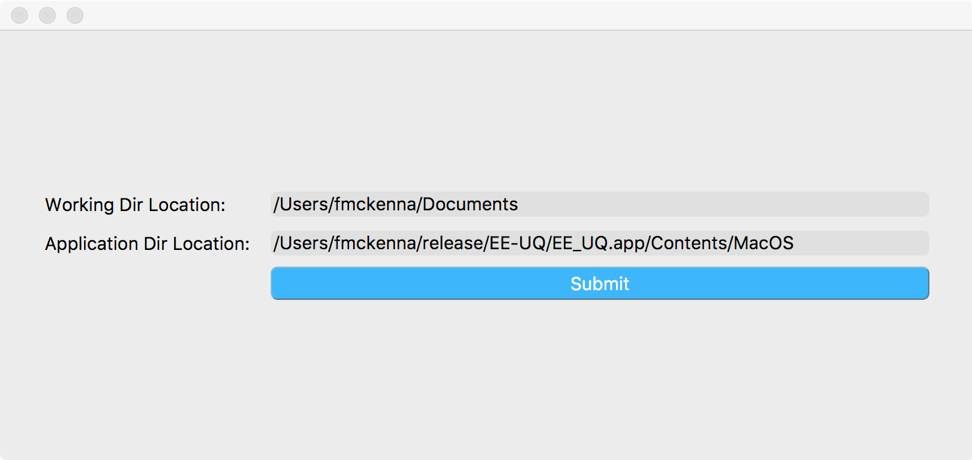
\includegraphics[width=0.8\textwidth]
    {usage/figures/runButton.png} }
  \caption{Pop-up shown after clicking \texttt{Run} button}
  \label{fig:figure15}
\end{figure}

The window that pops up is as shown in \autoref{fig:figure15}. There
are 2 entries and a push button:

\begin{itemize}
\item Working Dir Location: specifies where the \texttt{EE-UQ} application can create a “temporary” directory called tmp. SimCenter that the application 
creates when the submit button is pressed. The application creates
this directory, copies files to it that the application needs as a
result of your input (e.g. if you are using OpenSees input script, it
will to the tmp. SimCenter directory copy that script, ALL FILES IN
THAT DIRECTORY AND ALL FILES IN SUBDIRECTORIES OF THAT DIRECTORY GET
COPIED SO DON’T PLACE THE SCRIPT IN HOME, DOWNLOADS, DOCUMENTS, ….
\item Application Dir Location: SHOULD NOT BE TOUCHED unless you are introducing your own applications or want to build and modify the 
applications provided with the tool. It is this directory the
application tool looks to find the applications to run.
\end{itemize}


Finally, when inputs are finished the user hits submit button to start
the backend job. If it runs the window will close and the RES panel
will pop up on successful run. Do not press the submit button multiple
times while waiting for it to close. We cannot guarantee what will
happen and we did not disable the button in this release.

\subsection{RUN at DesignSafe}
Click this button to process the information, and send to DesignSafe
where the job will be run on a supercomputer and results stored in
your DesignSafe jobs folder.

\begin{figure}[!htbp]
  \centering {
    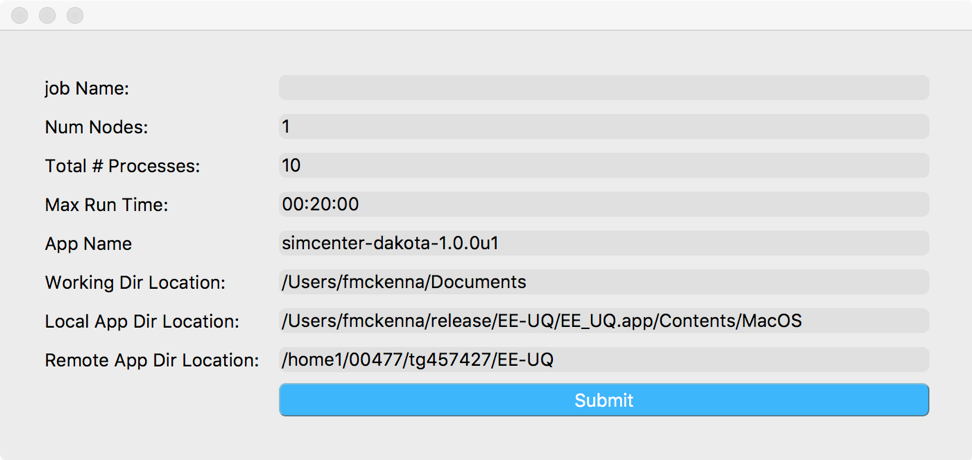
\includegraphics[width=0.8\textwidth]
    {usage/figures/remoteButton.png} }
  \caption{Pop-up shown after clicking \texttt{RUN at DesignSafe} button}
  \label{fig:remote_button}
\end{figure}

A similar bit longer input panel, shown in \autoref{fig:remote_button}
is brought up:
\begin{itemize}
\item JobName: The name the user can use to identify the job in Get from DesignSafe.
\item NumNodes: The number of compute nodes to use on Stampede2. Using the default App Name the job will run on Stampede2’s KNL Landing (KNL) 
compute nodes. Each node has 68 cores. The actual number of cores the
application will use on each of these nodes depends on the total
number of processes specified. As per the TACC webpage, for MPI tasks
it’s best not to specify more than 64-68 processes to run. Depending
on the numerical computations and amount of memory each uses, so as to
avoid page faulting, for large simulations you may wish to use more
nodes and less processes.
\item Total Number of Processes: Total number of MPI parallel processes the UQ engine is going to use.
\item Max Wall Time:  HOURS:MIN:SEC be conservative. Your job is killed after the time limit. On Stampede2 you have a max wall time of 24 hours.
\item App Name:   Name of Agave app to run. DO not touch unless you know what you are doing.
\item Working Dir Location: specifies where the \texttt{EE-UQ} application can create a “temporary” directory called tmp. SimCenter that the application 
creates when the submit button is pressed. The application creates
this directory, copies files to it that the application needs as a
result of your input (e.g. if you are using OpenSees input script, it
will to the tmp. SimCenter directory copy that script, ALL FILES IN
THAT DIRECTORY AND ALL FILES IN SUBDIRECTORIES OF THAT DIRECTORY. (SO,
DON’T PLACE THE SCRIPT IN HOME, DOWNLOADS, DOCUMENTS, …). That
directory is removed when jib has been successfully submitted.
\item Local App Dir Location: SHOULD NOT BE TOUCHED unless you are introducing your own applications or want to build and modify the applications 
provided with the tool. It is this directory the application tool
looks to find the applications it needs.
\item Remote App Dir Location: Remote directory on Stampede2 where applications needed by workflow reside. DO not touch unless you know what you are doing.

\end{itemize}

\subsection{GET from DesignSafe}
Click this button to obtain from DesignSafe your list of jobs and
select from that list a job to update status of, download or delete.

\subsection{Exit}
Click this button to exit the application. 
